\documentclass[12pt, letterpaper]{article} 
\usepackage[utf8]{inputenc}
\usepackage{setspace}
\usepackage[spanish]{babel} %pone en español textos automaticos
\usepackage{fancyhdr} % Se agrega el paquete fancyhdr
\usepackage{graphicx} % Se agrega el paquete graphicx
\usepackage{float} %para agregar imagenes con H
\usepackage{pdfpages} %agregar pdfs para datasheets y eso
\usepackage[a4paper, margin=3cm]{geometry} %marjenes y hoja A4


%pies de pagina
\pagestyle{fancy} % Se especifica el estilo de página como fancy
\fancyhf{} % Se limpian los encabezados y pies de página predefinidos
\rfoot{Página \thepage\ de \pageref{LastPage}} %texto derecha
\lfoot{Medidas Electrónicas I} %texto izquierda
%encabezado de pagina
\chead{UNIVERSIDAD TECNOLÓGICA NACIONAL - FRC} % centro
\fancyhead[R]{
\includegraphics[height=1cm]{imagenes/UTN_logo.jpg}}


\begin{document}

%Caratula
\begin{titlepage}
	\centering %texto centrado
	{
\includegraphics[width=0.2\textwidth]{imagenes/UTN_logo.jpg}\par}
	{\bfseries\LARGE Universidad Tecnológica Nacional \par}
	{\scshape\Large Facultad Regional Córdoba\par}
	\vspace{0.5cm}
	{\scshape\Huge Trabajo Práctico de laboratorio Nro. 3  \par}%titulo
	\raggedright %texto a la izquierda
	\vspace{0.5cm}
	{\Large Materia: Medidas Electrónicas 1 \par}%Materia
	\vspace{0.5cm}
	{\Large Curso: 4R1 \par}
	\vspace{0.5cm}
	{\Large Edificio: \par}%edificios
	\begin{itemize}
		\item{\Large Ingeniero Soro [Aula 606] \par}
		\item{\Large Laboratorio de electrónica \par}
	\end{itemize}
	\vspace{0.5cm}
	{\Large Profesores: \par} %profes
	\begin{itemize}
		\item{\Large [Teórico] Ing, Carlos Augusto Centeno \par}
		\item{\Large [Pratico] Ing, Luis Alberto Guanuco \par}
		\item{\Large [Práctico] Ing, Martin Alejandro Salamero \par}
	\end{itemize}
	\vspace{0.5cm}
	{\Large Autores: \par} %autores
	\begin{itemize}
		\item{\Large Pappano Meinardi, Joaquín - Leg.86730\par}
		\item{\Large Monteros Vigueras, Juan Manuel - Leg.86334\par}
		\item{\Large Romero Diaz, Agustín - Leg.86821\par}
	\end{itemize}
	\vspace{0.5cm}
	{\Large Fecha: {\today} \par}%pone fecha de hoy
\end{titlepage}

%Indice
\newpage
\tableofcontents
\newpage

%cuerpo documento
\section{Introducción}
En este trabajo práctico, se empleará métodos de mediciones instrumentos tipicos para la determinación de las principales características de una red de dos puertos (básicamente un amplificador). Los métodos que aquí ensayaremos abarcan ideas generales de gran interés en un amplio campo de las mediciones. Se verá, por ejemplo, la utilidad de las escalas en dB que poseen algunos instrumentos indagando en el uso de escalas en dBm 
 como dBu, y se implementará un método de substitución para medir una magnitud en forma indirecta Para este trabajo se empleará un amplificador de baja frecuencia que no tiene ninguna aplicación específica (figura \ref{fig:esq_amp}). Las medidas de este trabajo se realizaron sobre la probeta numero uno. 
\begin{figure}[H]
	\centering
	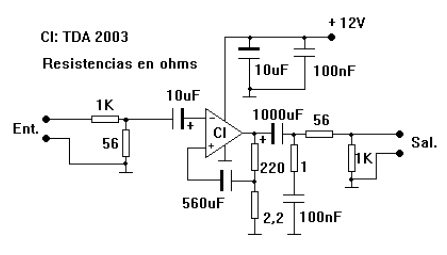
\includegraphics{imagenes/amplificador.png}
	\caption{Esquema Amplificador empleado}
    \label{fig:esq_amp}
\end{figure}

\subsection{Objetivo}
Determinar ciertas características de un amplificador (Impedancia de entrada y salida;
Ganancia de tensión y de potencia). Familiarizarse con las escalas en dB.

\subsection{Material e instrumental necesario}
\begin{itemize}
    \item Amplificador de baja frecuencia (figura \ref{fig:esq_amp}).
\item  Fuente de alimentación.
\item  Generador de señales con salida sinusoidal.
\item  Placa auxiliar con accesorios para las mediciones (figura \ref{fig:probeta}).
\item  Multímetro analógico con escala en dB (Preferentemente multímetro marca “UNIVO”).
\item  Multímetro digital.
\item Osciloscopio analogico  PS-200.
\end{itemize}

\begin{figure}[H]
	\centering
	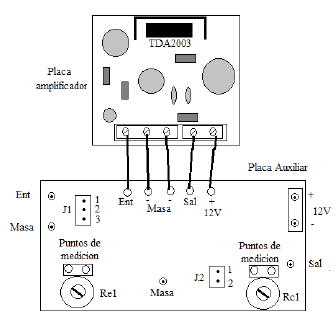
\includegraphics{imagenes/amplificador_placa_aux.png}
	\caption{Probeta completa}
    \label{fig:probeta}
\end{figure}

\section{Experiencia 1 "Medición de Zo"}

\subsection{Procedimiento}
%poner algun paso a paso del procedimiento
\begin{enumerate}
    \item Se alimenta el amplificador con 12v.
    \item A la entrada se introduce una señal senoidal de 1KKHz, para eso se coloca el jumper J1 conectando los puntos 1 y 2 esto deja sin carga de entrada al amplificador.
    \item Dejar desconectada la resistencia de carga Rc1 y poner la señal amplificada a máxima excursión simétrica, visualizando la salida en  un osciloscopio.
    \item Poner la resistencia Rc1, resistencia de carga, con el jumper J2 en los puntos 1 y 2.
    \item  Con el potenciómetro de carga Rc1 comenzar con el valor máximo del mismo para luego ajustarlo hasta que la lectura de la tensión de salida se reduzca a la mitad que la obtenida en vacío al principio.
    \item Desconectar la fuente de alimentación, abrir el jumper J2 y usar el multímetro digital para medir la impedancia de salida. Esta coincidirá con Z0 del amplificador.
      
\end{enumerate}
\begin{figure}[H]
	\centering
	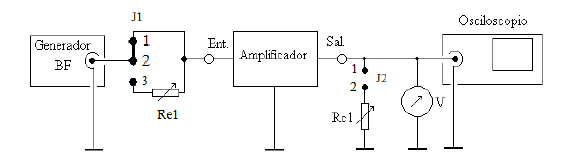
\includegraphics{imagenes/esquma_conec_E1.png}
	\caption{Esquema de conexión para experiencia 1}
    \label{fig:con_E1}
\end{figure}


\subsection{Valores obtenidos}

\begin{table}[H]
    \centering
    \caption{Valores obtenidos medida de Zo}
    \begin{tabular}{|c|c|c|c|}\hline
     frecuencia generador  & Valor nominal Zo & Vs sin Rc1 & $Rc1=Z0$ (para Vs'=Vs/2) \\\hline
     1KHz  & 50$\Omega$ & 10,20V & 49$\Omega$   \\ \hline   
    \end{tabular}
    \label{tab:Zo}
\end{table}

\section{Experiencia 2 "Medición de Zi"}

\subsection{Procedimiento}
%poner algun paso a paso del procedimiento
\begin{enumerate}
    \item  Repetir el primer paso de la experiencia anterior (con el Jumper J1 entre 1 y 2)
y anotar  valor de la tensión de salida.
\item  Jumper J1 entre 2 y 3, se intercala, en serie entre el generador y la entrada del amplificador, un resistor variable (Re1) cuidando de que el mismo se encuentre ajustado a su mínimo valor.
\item a aumentando el valor de Re1 hasta que la lectura de la tensión de salida se hace igual a la mitad de la que se obtuvo al principio.
\item Luego sacar el jumper J1, desconectar la fuente y medir con el voltímetro en ohm la impedancia de entrada.
\end{enumerate}

\begin{figure}[H]
	\centering
	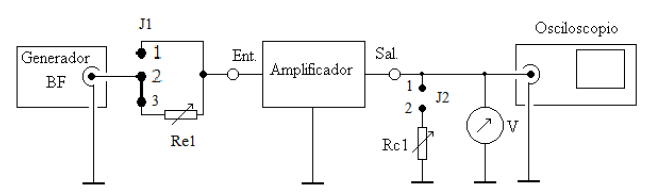
\includegraphics{imagenes/esquma_conec_E2.png}
	\caption{Esquema de conexión para experiencia 2}
    \label{fig:con_E2}
\end{figure}

\subsection{Valores obtenidos}

\begin{table}[H]
    \centering
    \caption{Valores obtenidos medida de Zi}
    \begin{tabular}{|c|c|c|c|}\hline
     frecuencia generador  & Valor nominal Zi & Vs sin Re1 & $Re1=Zi$ (para Vs'=Vs/2) \\\hline
     1KHz  & 1$K\Omega$ & 10,20V & 1144$\Omega$   \\ \hline   
    \end{tabular}
    \label{tab:Zi}
\end{table}


\section{Experiencia 3"Medición de Potencia de Salida Del Amplificador"}
\subsection{Procedimiento}
\begin{enumerate}
    \item Para la realización de esta experiencia, se realizo la calibración del multimetro digital UNIVO ajustando su la escala de dBu de la medición para ello se le coloco una tensión eficaz de 0,775V y se movió la aguja del mismo hasta que marcara 0dBu.
    \item   Se le introdujo al amplificador una Vs para que el mismo este en máxima excursión  simétrica con la carga Rc1 conectada a la salida , y con el multimetro en C.A en la escala de 3V se medio la salida en dbu.
    \item Como los dBu son una escala referida a voltaje normalizada para uno de 0775v, se llevo esta a dBm una escala referida a potencia mas específicamente mili Watts (mW).
    \item Con la potencia expresada en dBm se llevo esta a Watts (W), partiendo de que los dBm se encuentran normalizados para una potencia de 1mW. 
\end{enumerate}
\singlespacing

\subsection{Valores y cálculos}

Medición de Salida con carga $7.3dBu$ \singlespacing
\begin{equation*}
    dBm= dBU + 10*\log{\frac{600}{Rx}}
\end{equation*}
\singlespacing
Con el multimetro podemos ver los dBU, sin embargo estos instrumentos están calibrados para medir sobre cargas de $600\Omega$. Para que la medida obtenida sea equivalente a dBm al valor en dBu se le debe sumar una corrección
\singlespacing
\begin{equation*}
    \textbf{Correccion}=10*\log{\frac{600}{Rx}}
\end{equation*}
\singlespacing
Donde el valor de Rx corresponde al de la resistencia sobre el cual se efectúa la medición. en este caso Rc1 que es $49\Omega$
\singlespacing
\begin{equation*}
    &dBm= 7.3 + 10*\log{\frac{600}{49}=18.17dBm\singlespacing
    & dBm=10*\log{\frac{Px}{1mW}} \rightarrow Px=1mW*10^{\frac{dBm}{10}}\singlespacing
    &Px=1mW*10^{\frac{18.17}{10}}=65.75mW\singlespacing
\end{equation*}
\begin{table}[H]
    \centering
    \caption{Valores obtenidos Potencia de salida}
    \begin{tabular}{|c|c|}\hline
     Potencia salida en dBm  & Potencia salida en Watts\\\hline
     Ps= 18.17dBm  & Ps= 65.75mW = 0.06575W   \\ \hline   
    \end{tabular}
    \label{tab:Potencia}
\end{table} 




\section{Experiencia 4 "Medición de la ganancia de tensión y ganancia de potencia del 
amplificador"}
\subsection{Procedimiento}
\begin{enumerate}
    \item Se repiten los pasos de calibración del instrumento de la experiencia 3.
    \item Se meden la entrada del amplificador con el multimetro calibrado en la escala de 3V utilizando la unidad dBu.
    \item Se meden la salida del amplificador con el multimetro calibrado en la escala de 3V utilizando la unidad dBu.
    \item Se llevan las medidas tomadas en dBu a dBm, con estas podemos hacer referencia a ganancia de voltaje y de potencia respectivamente.
    \item Se calcula la ganancia en dB como la diferencia entre entrada y salida.
    \item Se lleva las ganancias en dB a una ganancia en veces. 
\end{enumerate}
\singlespacing 

\begin{figure}[H]
	\centering
	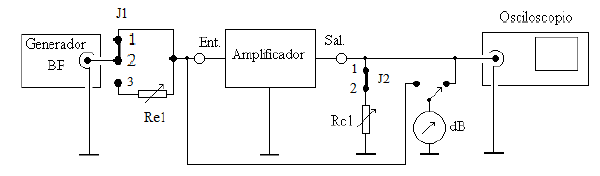
\includegraphics{imagenes/esquma_conec_E4.png}
	\caption{Esquema de conexión para experiencia 4}
    \label{fig:con_E4}
\end{figure}

\subsection{Valores y cálculos}

\begin{equation*}
    &dBU_{in}=1.3dBu \singlespacing
    &dBU_{out}=7.3dBu\singlespacing
\end{equation*}
La ganancia del amplificador la podemos ver como la diferencia de los dBU de salida con los de entrada. \singlespacing 
\begin{equation*}
    &Av_{dB}=dBU_{out} - dBU_{in}\singlespacing
    &Av_{dB}=7.3dBu - 1.3dBu=6dB\singlespacing
    &Av_{veces}=10^{\frac{Av_{db}}{20}}\singlespacing
    &Av_{veces}=10^{\frac{6}{20}}=1.99 veces\singlespacing
\end{equation*}
Esto también puede verse  aplicado a la potencia llevando todas nuestras mediciones y cálculos a una escala de dBm como se muestra a continuación. 
\singlespacing
\begin{equation*}
    &dBm_{in}= 1.3 + 10*\log{\frac{600}{11}}=-1.5dBm\singlespacing
    &dBm_{out}= 7.3 + 10*\log{\frac{600}{49}}=18.17dBm\singlespacing
    \singlespacing
    &Av_{dB}=dBm_{out} - dBm_{in}\singlespacing
    &Av_{dB}=18.17dBm - (-1.5dBm)=19.67dB\singlespacing
    &Av_{veces}=10^{\frac{Av_{db}}{20}}\singlespacing
    &Av_{veces}=10^{\frac{22.68}{20}}=9.62 veces\singlespacing
    
\end{equation*}

\begin{table}[H]
    \centering
    \caption{Valores obtenidos ganancia}
    \begin{tabular}{|c|c|c|c|c|}\hline
     Frecuencia generador  & Salida & Entrada & Ganancia en dB & Ganancia en veces\\\hline
     1KHz  & 7.3dBu &  1.3dBu & 6dB & 1.99veces \\ \hline  
    1KHz  & 18.17dBm &  -1.5dBm & 19.67dB & 9.62veces \\ \hline 
    \end{tabular}
    \label{tab:ganancia}
\end{table} 

\newpage
\section{Conclusión}
% Imploro suplico ruego que lo que diga aca responda a lo que pide el tp y más 
Se trabajo sobre un amplificador de usos múltiples el cual , en diferentes experiencias se midieron sus parámetros (Zi,Zo,Av,P), para esto se uso una placa auxiliar y deferentes elementos del laboratorio de electrónica, antes de la realización de las mediciones se realizaron  calibraciones, a los instrumentos analógicos de medición. En las mediciones 3 y 4, trabajamos sobre la escala en dbm, por lo cual la obtención de la potencia y la ganancia se pudo obtener de una manera más sencilla  
\singlespacing
En conclusión, al realizar mediciones de ganancia en dB utilizando un voltímetro, si fuera necesario cambiar el rango del mismo para medir, es importante tener en cuenta que se debe aplicar una corrección a las lecturas obtenidas. Esta corrección se debe basar en la relación entre los rangos utilizados, y se puede calcular utilizando la fórmula de conversión correspondiente $20 \log{F} \rightarrow$ donde F es la relación entre los rangos .
\singlespacing
Para la realización de mediciones con un multímetro digital, la ventaja que tenemos es que no necesitamos calibrarlo y en el caso de que sea de auto rango, como el que se puso probar,  no habría que cambiarle la escala. Las medidas se toman de forma directa en dBu, y al visualizar los valores de manera digital es menos probable que cometamos un error en la medición.  Sin embargo es importante saber si el instrumento esta calibrado o no para algún valor especifico de resistencia, generalmente 600$\Omega$, porque de ser así es necesario si medimos sobre una impedancia distinta aplicar el factor de corrección de resistencia del mismo modo que hacemos durante el trabajo con los dBu. 
\singlespacing
Los dbm son muy utilizados en el ámbito de las telecomunicaciones y en los amplificadores ya que se pueden transformar operaciones de producto en sumas y cocientes en restas, por eso  al medir con instrumentos que nos den su escala en db tenemos algunas ventajas.
\singlespacing
Estas ventajas incluyen la capacidad de medir grandes rangos de valores con una sola escala, la facilidad de realizar comparaciones entre diferentes valores de ganancia, y la posibilidad de realizar mediciones precisas y repetibles si se es precavido y se siguen los procedimientos.
\newpage

\section{Anexo}
\begin{figure}[H]
    \centering
    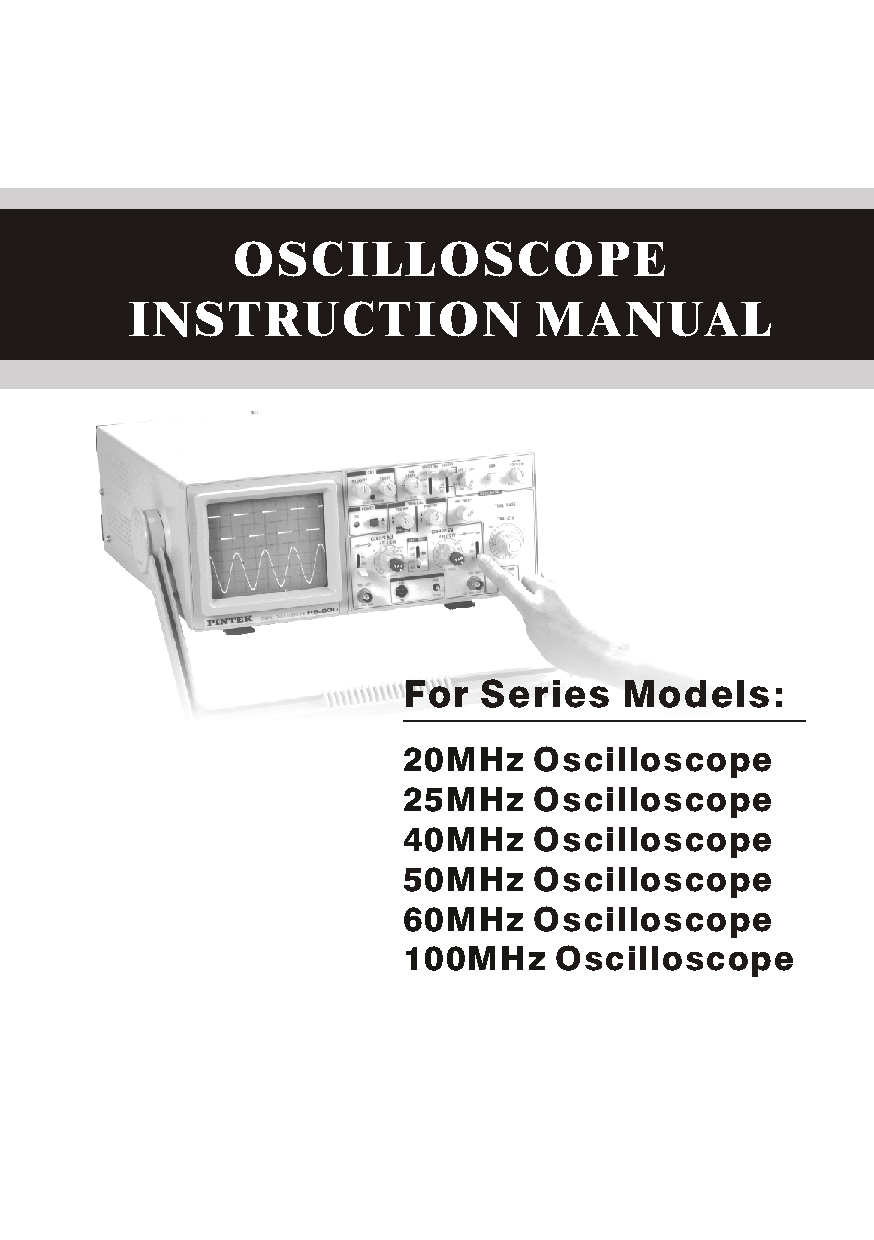
\includepdf[pages={1}, scale=0.60 ,pagecommand={\pagestyle{fancy}\fancyhf{}}]{imagenes/PS200.pdf}
\end{figure}
\newpage
\begin{figure}[H]
    \centering
    \includepdf[pages={8}, scale=0.60 ,pagecommand={\pagestyle{fancy}\fancyhf{}}]{imagenes/PS200.pdf}
\end{figure}
\newpage
\begin{figure}[H]
    \centering
    \includepdf[pages={9}, scale=0.60 ,pagecommand={\pagestyle{fancy}\fancyhf{}}]{imagenes/PS200.pdf}
\end{figure}
\newpage
\begin{figure}[H]
    \centering
    \includepdf[pages={10}, scale=0.60 ,pagecommand={\pagestyle{fancy}\fancyhf{}}]{imagenes/PS200.pdf}
\end{figure}




%no quitar del final
\label{LastPage}
\end{document}